% !TeX program = lualatex -synctex=1 -interaction=nonstopmode --shell-escape %.tex

\documentclass[_fin_decisions_lectures.tex]{subfiles}

\beamertemplatenavigationsymbolsempty


\subsection{Рыночная волатильность}
\begin{document}
\setbeamercovered{transparent}
\begin{frame}{Биномиальная модель оценки стоимости опционов}
\begin{itemize}
	\item
	Продавец и покупатель всегда имеют противоположные представления о развитии курса товара, лежащего в основе опциона. 
	\item
	Время в биномиальной модели распределено на периоды, например, дни, недели, месяцы. Курс на начало или конец периода может принимать только два значения: он может либо повысится, либо снизится на определенную процентную величину. 
	\item
	Биномиальная модель ничего не говорит о вероятности повышения или понижения курса базового актива за период.
\end{itemize}
\end{frame}

\begin{frame}{}
\begin{itemize}
\item
Цена опциона в конце срока обращения равна разнице между ценой исполнения и текущей ценой. Причем если получается отрицательная величина, то опцион не исполняется, т.е. его стоимость равна нулю. 
\item
Мы можем, пользуясь математическими параметрами изменения курса, спрогнозировать наиболее вероятный диапазон изменения котировок в течении всего срока обращения опциона. 
\end{itemize}
\end{frame}

\setbeamercovered{invisible}
\begin{frame}[shrink=15]{Изменения котировок USDRUB c 01.10.2013 по 01.10.2014}
\begin{center}
% Table generated by Excel2LaTeX from sheet 'USDRUB'
\begin{table}[htbp]
  \centering
    \begin{tabular}{>{\onslide<1->}c
    				>{\onslide<1->}c        
    				>{\onslide<2->}c}
    \toprule
    \multicolumn{1}{c}{Дата} & \multicolumn{1}{c}{Цена закрытия} & \multicolumn{1}{c}{$\Delta,\%$} \\
    \midrule
    01.10.2013 & 32,0973 &  \\
    01.11.2013 & 33,0852 & 3,08\% \\
    01.12.2013 & 32,8311 & -0,77\% \\
    01.01.2014 & 35,2523 & 7,37\% \\
    01.02.2014 & 35,9238 & 1,90\% \\
    01.03.2014 & 35,1707 & -2,10\% \\
    01.04.2014 & 35,6287 & 1,30\% \\
    01.05.2014 & 34,8855 & -2,09\% \\
    01.06.2014 & 33,9675 & -2,63\% \\
    01.07.2014 & 35,705 & 5,12\% \\
    01.08.2014 & 37,1041 & 3,92\% \\
    01.09.2014 & 39,5562 & 6,61\% \\
    01.10.2014 & 42,9913 & 8,68\% \\
    \bottomrule
    \end{tabular}%
  \label{tab:addlabel}%
\end{table}%
\end{center}
\end{frame}
\begin{frame}{График котировок USDRUB по месяцам}
\begin{center}
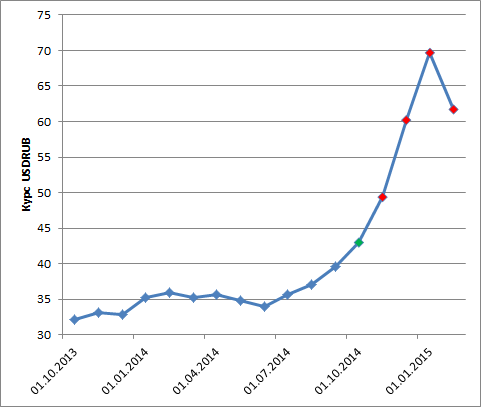
\includegraphics[scale=0.7]{img/usdrubquoteschart}
\end{center}
\end{frame}
\begin{frame}{Процентное изменение котировок USDRUB по месяцам}
\begin{center}
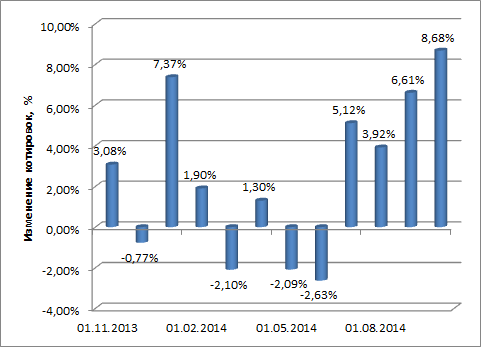
\includegraphics[scale=0.8]{img/usdrubdeltaperc}
\end{center}
\end{frame}
\begin{frame}{Интервалы процентных изменений котировок  USDRUB}
\begin{center}
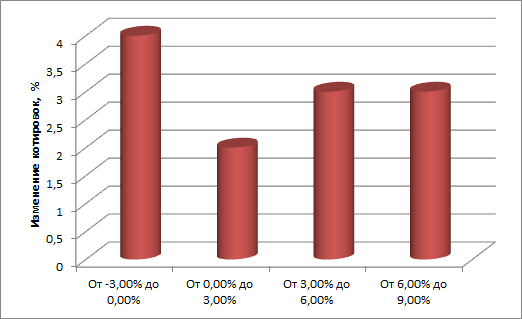
\includegraphics[scale=0.8]{img/usdrubquotesintervals}
\end{center}
\end{frame}
\setbeamercovered{transparent}
\begin{frame}{Формулы для расчета средней и стандартного отклонения}
\begin{itemize}[<+->]
\item
Среднее значение доходности:
$$m=\frac{\sum_{i=1}^n x_i}{n}$$
где $x_i$ – наблюденное значение;

$n$ – количество наблюдений.
\item
Стандартное отклонение:
$$s=\sqrt{\frac{\sum_{i=1}^n (m-x_i)^2}{n-1}}$$
\end{itemize}
\end{frame}
\setbeamercovered{invisible}
\begin{frame}[shrink=15]{Среднее ежемесячное изменение котировок USDRUB и его стандартное отклонение}
% Table generated by Excel2LaTeX from sheet 'Расчет m и s'
\begin{table}[htbp]
  \centering
    \begin{tabular}{cccc}
    \toprule
    & $x_i$    & $m-x_i$  & $(m-x_i)^2$ \\
    \midrule
1 & 3,08\% & \hiddencell{4}{-0,54\%} & \hiddencell{5}{0,30} \\
2 & -0,77\% & \hiddencell{4}{3,30\%} & \hiddencell{5}{10,90} \\
3 & 7,37\% & \hiddencell{4}{-4,84\%} & \hiddencell{5}{23,44} \\
4 & 1,90\% & \hiddencell{4}{0,63\%} & \hiddencell{5}{0,40} \\
5 & -2,10\% & \hiddencell{4}{4,63\%} & \hiddencell{5}{21,44} \\
6 & 1,30\% & \hiddencell{4}{1,23\%} & \hiddencell{5}{1,52} \\
7 & -2,09\% & \hiddencell{4}{4,62\%} & \hiddencell{5}{21,34} \\
8 & -2,63\% & \hiddencell{4}{5,17\%} & \hiddencell{5}{26,68} \\
9 & 5,12\% & \hiddencell{4}{-2,58\%} & \hiddencell{5}{6,66} \\
10 & 3,92\% & \hiddencell{4}{-1,38\%} & \hiddencell{5}{1,92} \\
11 & 6,61\% & \hiddencell{4}{-4,08\%} & \hiddencell{5}{16,61} \\
12 & 8,68\% & \hiddencell{4}{-6,15\%} & \hiddencell{5}{37,83} \\
    \midrule
    $\Sigma$& \hiddencell{2}{30,40\%} 
    &  - 
    & \onslide<6->{169,02} \\
    \textbf{m}
    & \hiddencell{3}{\textit{\textbf{2,5337\%}}} 
    & \textbf{s}
    & \hiddencell{7}{\textit{\textbf{3,9199\%}}} \\
    \bottomrule
    \end{tabular}%
  \label{tab:addlabel}%
\end{table}%

\end{frame}
\begin{frame}{Средняя ежемесячная доходность USDRUB и ее стандартное отклонение}
\begin{center}

% Table generated by Excel2LaTeX from sheet 'Расчет m и s'
\begin{table}[htbp]
  \centering
    \begin{tabular}{lr}
    \toprule
    m     & 2,5337\% \\
    s     & 3,9199\% \\
    \midrule
    m+s   & 6,4535\% \\
    m-s   & -1,3862\% \\
    \midrule
    u     & 1,0645 \\
    d     & 0,9861 \\
    \bottomrule
    \end{tabular}%
  \label{tab:addlabel}%
\end{table}%
\end{center}
\end{frame}
\subsection{Дерево цен}
\begin{frame}{Построение дерева цен}
{Параметры опционов колл и пут}
\begin{center}
% Table generated by Excel2LaTeX from sheet 'Модель'
\begin{table}[htbp]
  \centering
    \begin{tabular}{lrr}
    \toprule
    & \multicolumn{2}{c}{Тип опциона} \\  \cmidrule{2-3}
    & Колл & Пут \\
    \midrule
    Цена исполнения  & 45,00 ~₽ & 45,00 ~₽ \\
    Срок  & 2 месяца & 2 месяца \\
    Ставка USD, \% год-х & 1\% & 1\% \\
    Ставка RUB, \% год-х & 8,00\% & 8,00\% \\
    Ставка USD, \% мес. & 0,08\% & 0,08\% \\
    Ставка RUB, \% мес. & 0,67\% & 0,67\% \\
    \bottomrule
    \end{tabular}%
  \label{tab:addlabel}%
\end{table}%
\end{center}
\end{frame}
\setbeamercovered{invisible}
\begin{frame}[fragile]{Бинарное дерево}
\begin{figure}
	\center
	\begin{overprint}
		\forloop{slideno}{1}{\value{slideno} < 7}{%
			\only<\value{slideno}>{
				\includegraphics[page=\value{slideno},
				scale=0.8
				% trim={<left> <lower> <right> <upper>}				
				,trim={0cm 2cm 0cm 0cm}
				,clip]
				{tikz/price_binary_tree}}}
	\end{overprint}
	\caption{Бинарное дерево цен}
\end{figure}
\end{frame}

\begin{frame}[fragile]{Бинарное дерево}
\begin{figure}
	\center
	\begin{overprint}
		\forloop{slideno}{1}{\value{slideno} < 4}{%
			\only<\value{slideno}>{
				\includegraphics[page=\value{slideno},
				scale=0.8
				% trim={<left> <lower> <right> <upper>}				
				,trim={0cm 2cm 0cm 0cm}
				,clip]
				{tikz/price_binary_tree_full}}}
	\end{overprint}
	\caption{Стоимость опционов в конце срока}
\end{figure}

\end{frame}
\subsection{Стоимость опциона в промежуточные периоды}
\setbeamercovered{transparent}
\begin{frame}{}
\begin{itemize}[<+->]
\item
Цена опциона в промежуточные периоды определяется путем составления и расчета эквивалентного портфеля. Т.е. портфеля, состоящего из определенного количества базового актива и денег, стоимость которого в любой момент времени равна стоимости опциона на базовый актив.
\item
Зная стоимость опциона на конец рассматриваемого периода и решив систему уравнений мы можем определить стоимость опциона на начало периода и т.д. до дня предполагаемой покупки. Это и будет теоретически справедливая цена опциона.

\end{itemize}
\end{frame}
\begin{frame}{}
\begin{itemize}[<+->]
\item
При расчете стоимости опционов предполагается, что денежная часть эквивалентного портфеля приносит некоторый безрисковый доход, в случае длинной позиции по деньгам (опцион пут) или расход, в случае короткой позиции по деньгам (опцион колл). 
\item
Для расчета принимаем процентную ставку по государственным облигациям США.
\end{itemize}
\end{frame}
\setbeamercovered{invisible}
\begin{frame}[shrink=10]{Пример расчета первой промежуточной цены опциона}
\begin{align*}
\begin{cases} 
\onslide<2->{z_1 = 45,7658 \cdot x_1 + y_1}\\ 
\onslide<3->{3,7193 = 48,7193 \cdot x_1 \cdot (1 + r_{USD}) + y_1 \cdot (1 + r_{RUB})}\\
\onslide<4->{0,1314 = 45,1314 \cdot x_1 \cdot (1 + r_{USD}) + y_1 (1 + \cdot r_{RUB})}
\end{cases}
\end{align*}
$z_1$ – промежуточная цена опциона (искомая величина);

$x_1$ – количество базового актива в портфеле (базовой валюты) отрицательное значение означает короткую позицию;

$y_1$ – количество валюты котировки в портфеле отрицательное значение означает короткую позицию;

$r_{USD},r_{RUB}$ – процентная ставка без риска по займам/депозитам, соответственно, в базовой валюте и валюте котировки, годовых.
\end{frame}
\setbeamercovered{transparent}
\begin{frame}{}
\begin{itemize}[<+->]
\item
При расчетах цены опционов колл и пут используются одинаковые формулы. Различия есть только при определении цены опциона в конце срока обращения (при вычислении  разницы между текущей котировкой базового актива и ценой исполнения опциона).
\item
Промежуточная цена опциона, иногда бывает недостаточно большой, чтобы удержать владельца опциона от его исполнения, в этом случае, в качестве промежуточной цены опциона используется прибыль от его исполнения на рассматриваемую дату.
\end{itemize}
\end{frame}
\setbeamercovered{invisible}
\subsection{Стоимость опциона колл и пут}
\begin{frame}[fragile]{Опцион колл}

\begin{figure}
	\center
	\begin{overprint}
		\forloop{slideno}{1}{\value{slideno} < 6}{%
			\only<\value{slideno}>{
				\includegraphics[page=\value{slideno},
				scale=0.8
				% trim={<left> <lower> <right> <upper>}				
				,trim={0cm 2cm 0cm 0cm}
				,clip]
				{tikz/option_call}}}
	\end{overprint}
	\caption{Опцион колл}
\end{figure}

\end{frame}
\begin{frame}[fragile]{Опцион пут}

\begin{figure}
	\center
	\begin{overprint}
		\forloop{slideno}{1}{\value{slideno} < 8}{%
			\only<\value{slideno}>{
				\includegraphics[page=\value{slideno},
				scale=0.8
				% trim={<left> <lower> <right> <upper>}				
				,trim={0cm 2cm 0cm 0cm}
				,clip]
				{tikz/option_put}}}
	\end{overprint}
	\caption{Опцион пут}
\end{figure}

\end{frame}
\subsection{Стоимость бинарных опционов}
\begin{frame}{Стоимость бинарных опционов}
{Параметры бинарных опционов}
\begin{center}

% Table generated by Excel2LaTeX from sheet 'Модель'
\begin{table}[htbp]
  \centering
    \begin{tabular}{lrr}
    \toprule
    & \multicolumn{2}{c}{Тип опциона} \\  \cmidrule{2-3}
    & 1 касание & б/ касаний \\
    \midrule
    Барьерная цена & 48,00 ~₽ & 42,50 ~₽ \\
    Выплата & \$1 000 & \$1 000 \\
    Срок  & 2 месяца & 2 месяца \\
    Ставка USD, \% год-х & 1\% & 1\% \\
    Ставка RUB, \% год-х & 8,00\% & 8,00\% \\
    Ставка USD, \% мес. & 0,08\% & 0,08\% \\
    Ставка RUB, \% мес. & 0,67\% & 0,67\% \\
    \bottomrule
    \end{tabular}%
  \label{tab:addlabel}%
\end{table}%
\end{center}
\end{frame}
\begin{frame}[fragile]{Опцион в одно касание}
\begin{figure}
	\center
	\begin{overprint}
		\forloop{slideno}{1}{\value{slideno} < 9}{%
			\only<\value{slideno}>{
				\includegraphics[page=\value{slideno},
				scale=0.8
				% trim={<left> <lower> <right> <upper>}				
				,trim={0cm 2cm 0cm 0cm}
				,clip]
				{tikz/option_one_touch}}}
	\end{overprint}
	\caption{Опцион в одно касание}
\end{figure}
\end{frame}
\begin{frame}[fragile]{Опцион без касаний}
\begin{figure}
	\center
	\begin{overprint}
		\forloop{slideno}{1}{\value{slideno} < 9}{%
			\only<\value{slideno}>{
				\includegraphics[page=\value{slideno},
				scale=0.8
				% trim={<left> <lower> <right> <upper>}				
				,trim={0cm 2cm 0cm 0cm}
				,clip]
				{tikz/option_no_touch}}}
	\end{overprint}
	\caption{Опцион в без касаний}
\end{figure}
\end{frame}
\setbeamercovered{transparent}
\subsection{Общая однопериодная модель}
\begin{frame}{Общая однопериодная модель}
\begin{figure}
	\center
	\begin{overprint}
		\forloop{slideno}{1}{\value{slideno} < 2}{%
			\only<\value{slideno}>{
				\includegraphics[page=\value{slideno},
				scale=0.8
				% trim={<left> <lower> <right> <upper>}				
				,trim={0cm 7cm 0cm 0cm}
				,clip]
				{tikz/option_general_model}}}
	\end{overprint}
	\caption{Общая однопериодная модель}
\end{figure}
\end{frame}
\begin{frame}
где
$S$ - текущая цена базового актива;

$E$ - цена исполнения опциона.
\begin{align}
C_u = \begin{cases} u \cdot S - E, & \mbox{для случая } u \cdot S > E \\ 
0, & \mbox{для случая } u \cdot S \leq E \end{cases}\\
C_d = \begin{cases} d \cdot S - E, & \mbox{для случая } d \cdot S > E \\ 
0, & \mbox{для случая } d \cdot S \leq E \end{cases}
\end{align}
\end{frame}
\begin{frame}[shrink=15]{Система уравнений\\для однопериодной модели}{и ее решение}
\begin{align}
\begin{cases} 
C = S \cdot x + y\\ 
C_u = u \cdot S \cdot x \cdot r_{USD} + y \cdot r_{RUB}\\
C_d = d \cdot S \cdot x \cdot r_{USD} + y \cdot r_{RUB}
\end{cases}\\[12pt]
x=\frac{C_u-C_d}{(u-d)\cdot S \cdot r_{USD}}
y=\frac{u \cdot C_d-d \cdot C_u}{(u-d) \cdot r_{RUB}}
\end{align}
\begin{align}
C = S \cdot x + y
\end{align}

где

$x, y$ - размеры позиций, соответственно, в долларах и рублях;

$r_{USD},r_{RUB}$ - процентные ставки по заимствованию (кредитованию) за период времени \textit{T}, соответственно, в долларах и рублях.
\end{frame}

\subsection{Контрольные вопросы}
\begin{frame}[allowframebreaks]{Контрольные вопросы}
1. Понятие биномиальной модели оценки стоимости опционов.

2. Построение дерева цен в биномиальной модели оценки стоимости опционов.

3. Определение стоимости опционов в промежуточные периоды в биномиальной модели оценки стоимости опционов.

4. Оценка опционов колл посредством биномиальной модели.

\pagebreak
5. Оценка опционов пут посредством биномиальной модели.

6. Оценка бинарных опционов в одно касание посредством биномиальной модели.

7. Оценка бинарных опционов без касаний посредством биномиальной модели.

8. Математическое определение общей однопериодной биномиальной модели оценки стоимости опционов.
\end{frame}

\end{document}